\documentclass{beamer}
\mode<presentation>
\usepackage{amsmath}
\usepackage{amssymb}
\usepackage{adjustbox}
\usepackage{subcaption}
\usepackage{enumitem}
\usepackage{multicol}
\usepackage{mathtools}
\usepackage{listings}
\usepackage{url}
\usepackage{gvv}
\def\UrlBreaks{\do\/\do-}
\usetheme{Boadilla}
\usecolortheme{lily}
\setbeamertemplate{footline}
{
  \leavevmode%
  \hbox{%
  \begin{beamercolorbox}[wd=\paperwidth,ht=2.25ex,dp=1ex,right]{author in head/foot}%
    \insertframenumber{} / \inserttotalframenumber\hspace*{2ex} 
  \end{beamercolorbox}}%
  \vskip0pt%
}
\setbeamertemplate{navigation symbols}{}

\title{Solving Linear Equations}
\author{Dwarak A - EE24BTECH11019}
\date{\today} 

\begin{document}

\begin{frame}
\titlepage
\end{frame}

\section*{Outline}
\begin{frame}
\tableofcontents
\end{frame}

\section{Problem Statement}
\begin{frame}
\frametitle{Problem Statement}
Solve the following pair of linear equations:
\begin{align}
    \frac{3x}{2} - \frac{5y}{3} &= -2 \\
    \frac{x}{3} + \frac{y}{2} &= \frac{13}{6}
\end{align}
\end{frame}

\section{Solution}
\subsection{Matrix Representation}
\begin{frame}
\frametitle{Matrix Representation}
Let
\begin{align}
    \vec{x} = \myvec{x \\ y}
\end{align}
Expressing the system in matrix form:
\begin{align}
    \myvec{\frac{3}{2} & \frac{-5}{3}\\ \frac{1}{3} & \frac{1}{2}}\vec{x} &= \myvec{-2\\\frac{13}{6}} \\
    \myvec{9 & -10 \\ 2 & 3}\vec{x} &= \myvec{-12 \\ 13} \\
    A\vec{x} &= \vec{b}
\end{align}
\end{frame}

\subsection{LU Decomposition}
\begin{frame}
\frametitle{LU Decomposition}
Any non-singular matrix $A$ can be expressed as a product of a lower triangular matrix $L$ and an upper triangular matrix $U$, such that
\begin{align}
    A &= LU\\
    \implies LU\vec{x} &= \vec{b}
\end{align}
$U$ is determined by row reducing $A$ using a pivot:
\begin{align}
    \myvec{9 & -10\\2 & 3} \xrightarrow{R_2 \to R_2 - \frac{2}{9}R_1} \myvec{9 & -10\\0 & \frac{47}{9}}
\end{align}
Thus,
\begin{align}
    U = \myvec{9 & -10\\0 & \frac{47}{9}}
\end{align}
\end{frame}

\begin{frame}
\frametitle{LU Decomposition}
Let 
\begin{align}
    L = \myvec{1 & 0\\l & 1}
\end{align}
$l$ is the multiplier used to zero out $a_{21}$ in $A$:
\begin{align}
    L = \myvec{1 & 0\\ \frac{2}{9} & 1}
\end{align}
\end{frame}

\subsection{Update Equations}
\begin{frame}
\frametitle{Update Equations}
This $LU$ decomposition could also be computationally found using Doolittle's algorithm. The update equations are given by:
\begin{align}
    U_{ij} &= \begin{cases}
        A_{ij} & \quad i = 0\\
        A_{ij} - \sum_{k = 0}^{i - 1} L_{ik} U_{kj} & \quad i > 0
    \end{cases}\\
    L_{ij} &= \begin{cases}
        \frac{A_{ij}}{U_{jj}} & \quad j = 0, U_{jj} \neq 0\\
        \frac{A_{ij} - \sum_{k = 0}^{j - 1} L_{ik} U_{kj}}{U_{jj}} & \quad j > 0
    \end{cases}
\end{align}
\end{frame}


\subsection{Forward and Back Substitution}
\begin{frame}
\frametitle{Two-Step Solution Process}
We can get the solution to our problem by the two-step process:
\begin{align}
    L\vec{y} &= \vec{b}\\
    U\vec{x} &= \vec{y}
\end{align}
\end{frame}

\begin{frame}
\frametitle{Forward Substitution}
To solve $L\vec{y} = \vec{b}$, use forward substitution:
\begin{align}
    \myvec{1 & 0\\ \frac{2}{9} & 1}\myvec{y_1 \\ y_2} &= \myvec{-12 \\ 13}\\
    \myvec{y_1 \\ y_2} &= \myvec{-12 \\ \frac{47}{3}}
\end{align}
\end{frame}

\begin{frame}
\frametitle{Back Substitution}
To solve $U\vec{x} = \vec{y}$, use back substitution:
\begin{align}
    \myvec{9 & -10\\ 0 & \frac{47}{9}}\myvec{x_1 \\ x_2} &= \myvec{-12 \\ \frac{47}{3}}\\
    \myvec{x_1 \\ x_2} &= \myvec{2 \\ 3}
\end{align}
\end{frame}

\section{Visualization}
\begin{frame}
\frametitle{Plot}
\begin{figure}[H]
    \centering
    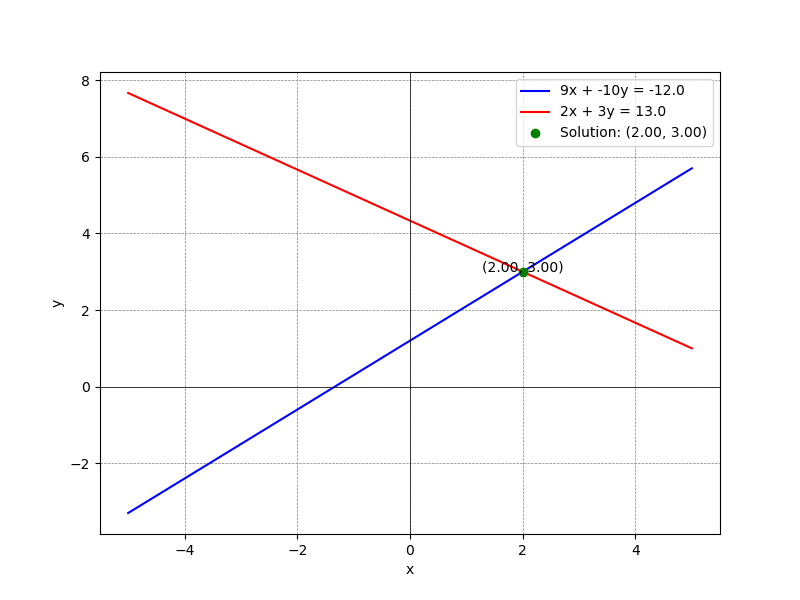
\includegraphics[width=0.7\textwidth]{figs/plot.png}
    \caption{Graphical solution of the linear equations}
\end{figure}
\end{frame}

\end{document}

